\section{Integral Theorems and Vector Analysis}
\begin{marginfigure}
	\begin{center}
	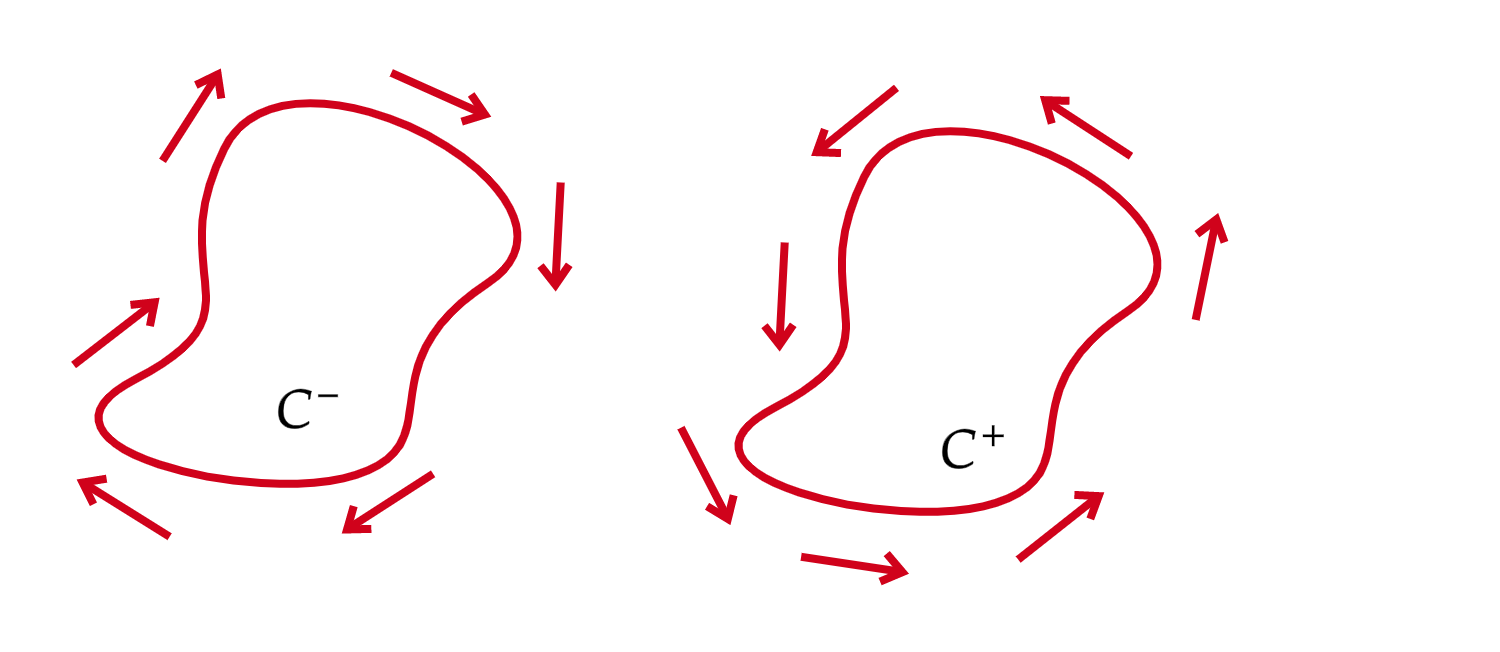
\includegraphics[width=\linewidth]{figures/wk-7/fig-1.png}
	\end{center}
\end{marginfigure}


\subsection{Green's and Stokes' Theorem}
In this section, we will relate a line integral along a closed curve $C$ in the plane to a double integral over the region enclosed by the curve. 

\begin{thm}[Green's Theorem]
	Let $D$ be a simple region with an oriented piecewise continuous boundary $C^+$. Suppose that $P: D \rightarrow \R$ and $Q: D \rightarrow \R$ are of class $C^1$. Then,
	\[\oint_{C^+} P d x+Q d y=\iint_D\left(\frac{\partial Q}{\partial x}-\frac{\partial P}{\partial y}\right) d x d y\]
\end{thm}

\hfill

\begin{rmk}
	If $\mathbf{F} = \mathbf{\nabla} V$ is conservative, then $\mathbf{\nabla} \times \mathbf{F} = 0$. Since,
	\[
	\mathbf{\nabla} \times \mathbf{F}=\left|\begin{array}{ccc}
	\mathbf{i} & \mathbf{j} & \mathbf{k} \\
	\partial_x & \partial_y & \partial_z \\
	P(x, y) & Q(x, y) & 0
	\end{array}\right| = 0 \cdot \mathbf{i} + 0 \cdot \mathbf{j} + \left(\frac{\partial Q}{\partial x} - \frac{\partial P}{\partial y}\right) \cdot \mathbf{k}
	\]
	Green's Theorem quantifies the amount by which  $\mathbf{F}$ fails to be conservative by relating the two integrals:
	\[\oint_{{(\partial D)}^+} \mathbf{F} \cdot d \mathbf{s} \quad \text{ and } \quad \iint_D\left(\frac{\partial Q}{\partial x}-\frac{\partial P}{\partial y}\right) d x d y\]
\end{rmk}

\hfill

\noindent The corollary of the previous remark is not true.

\hfill

\begin{rmk}
	If $\mathbf{\nabla} \times \mathbf{F} = 0$, then $\mathbf{F}$ is not necessarily conservative.
\end{rmk}

\begin{proof}
	Consider the vector field $\mathbf{F}$ defined on $U = \R^2 - \{(0,0)\}$:
	\[\mathbf{F}=\frac{-y}{x^2+y^2} \cdot \mathbf{i}+\frac{x}{x^2+y^2} \cdot \mathbf{j}\]
	We will verify that $\mathbf{\nabla} \times \mathbf{F} = 0$ everywhere on $U$.
	\[\mathbf{\nabla} \times \mathbf{F} = (Q_x - P_y) \cdot \mathbf{k}\]
	Observe that $P_x = Q_y$ for all $x, y \in U$.
	\[Q_x = \frac{-x^2 + y^2}{x^2+y^2} \quad \text{ and } \quad P_y = \frac{-x^2+y^2}{(x^2+y^2)^2}\]
	It follows that $(Q_x - P_y) \cdot \mathbf{k} = 0$. However, $\mathbf{F}$ was carefully chosen \textbf{not} to be conservative. Assume for a contradiction that $\mathbf{F}$ is conservative. The line integral must satisfy that,
	\[\oint_{\mathbf{c}} \mathbf{F} \cdot d \mathbf{s} = 0\]
	for any choice of closed curve $\mathbf{c}(t)$. Take the unit circle $\mathbf{c}(t) = (\cos t, \sin t)$ where $0 \leq t \leq 2\pi$.  We obtain,
	\[\oint_{\mathbf{c}} \mathbf{F} \cdot d \mathbf{s} = \int_{0}^{2\pi} d t \neq 0\]
\end{proof}

\hfill 

\noindent There is more to learn from this counter-example. 

\hfill 

\begin{ex}{Visualizing the vector field $\mathbf{F}$}{label}
	The vector field $\mathbf{F}=\frac{-y}{x^2+y^2} \cdot \mathbf{i}+\frac{x}{x^2+y^2} \cdot \mathbf{j}$ can be visualized as,

	\hfill

	\begin{center}
	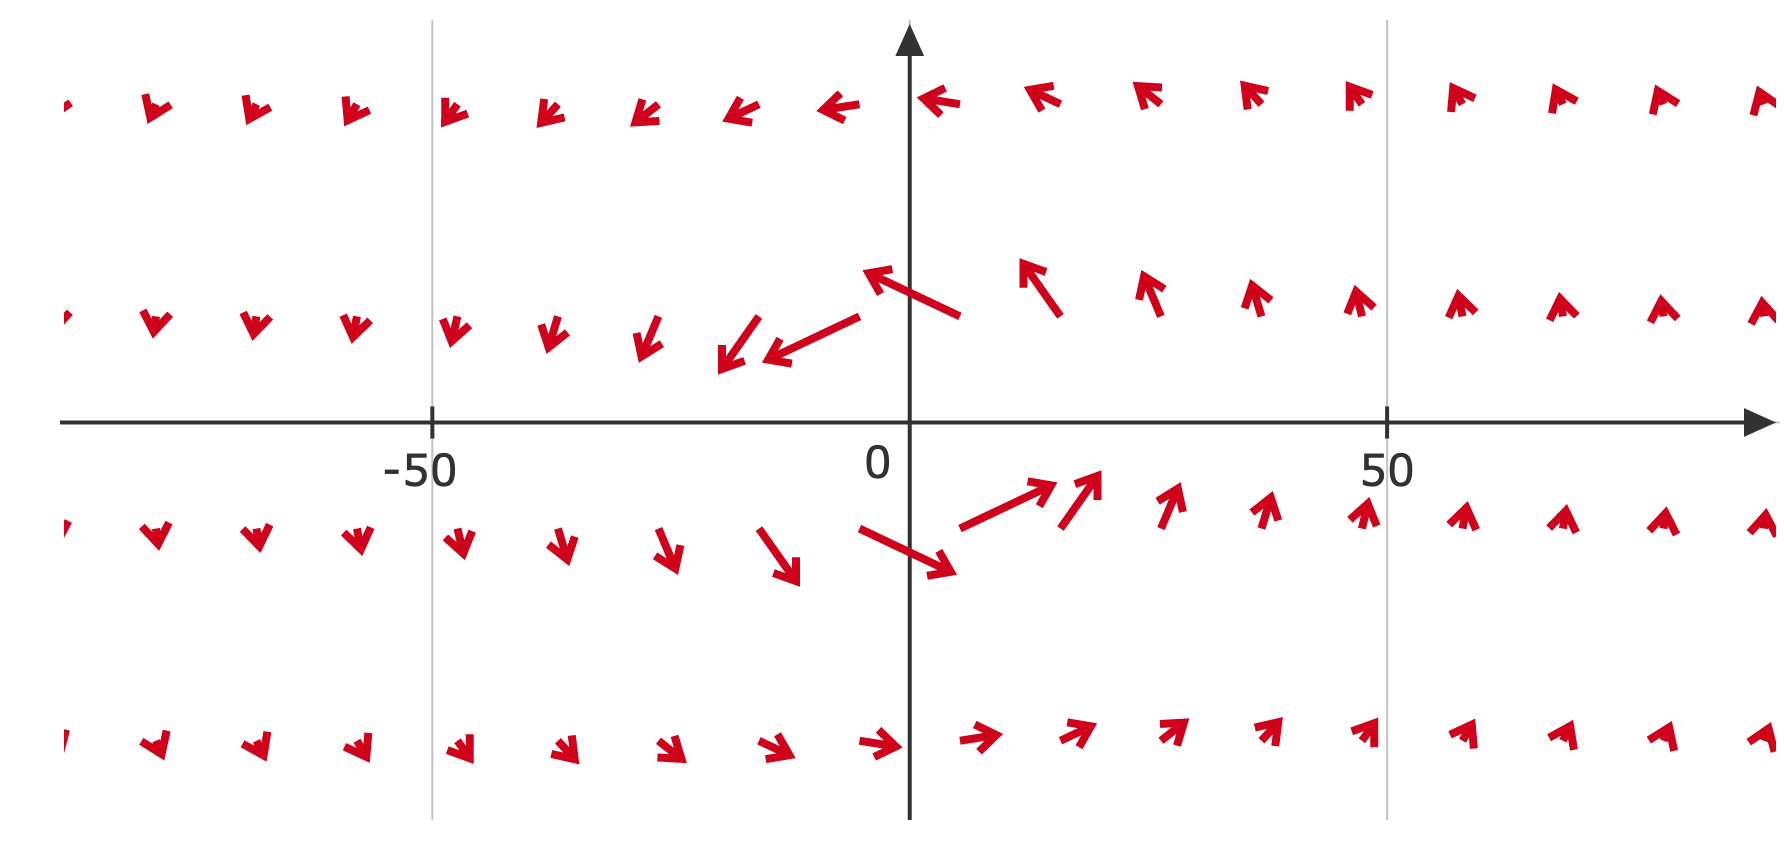
\includegraphics[width=\linewidth]{figures/wk-7/fig-3.png}
	\end{center}

\end{ex}

\hfill 

\begin{rmk}
	Let $\mathbf{c}(t)$ be an arbitrary closed curve. Consider
	\[\mathbf{F}=\frac{-y}{x^2+y^2} \cdot \mathbf{i}+\frac{x}{x^2+y^2} \cdot \mathbf{j}\]
	If $\mathbf{c}(t)$ contains $(0,0)$ in its interior, then,
	\[\oint_{\mathbf{c}} \mathbf{F} \cdot d \mathbf{s} = 2 \pi\]
	Otherwise,
	\[\oint_{\mathbf{c}} \mathbf{F} \cdot d \mathbf{s} = 0\]
\end{rmk}

\begin{marginfigure}
	Let $D$ be a region in $\R^2$ containing the origin. There exists $r > 0$ such that $D_r(\mathbf{0}) \subseteq D$. The area of $B_r$ is $2\pi$, implying that the line integral evaluates to $2\pi$ since the remaining work is 0 by the previous calculation:
	\[\iint_{D - D_r(\mathbf{0})} \underbrace{\left(Q_x-P_y\right)}_{=0}dx d y=0\]
\end{marginfigure}

\hfill 

\noindent It is possible for the region $D$ to contain holes, in which case there are multiple boundary curves. In this case, we write:
\[\oint_{\partial D^{+}} \mathbf{F} \cdot d \mathbf{s}=\oint_{\partial D_1^{+}} \mathbf{F} \cdot d \mathbf{s}+\oint_{\partial D_2^{+}} \mathbf{F} \cdot d \mathbf{s}\]

\hfill

\begin{marginfigure}
	\begin{center}
	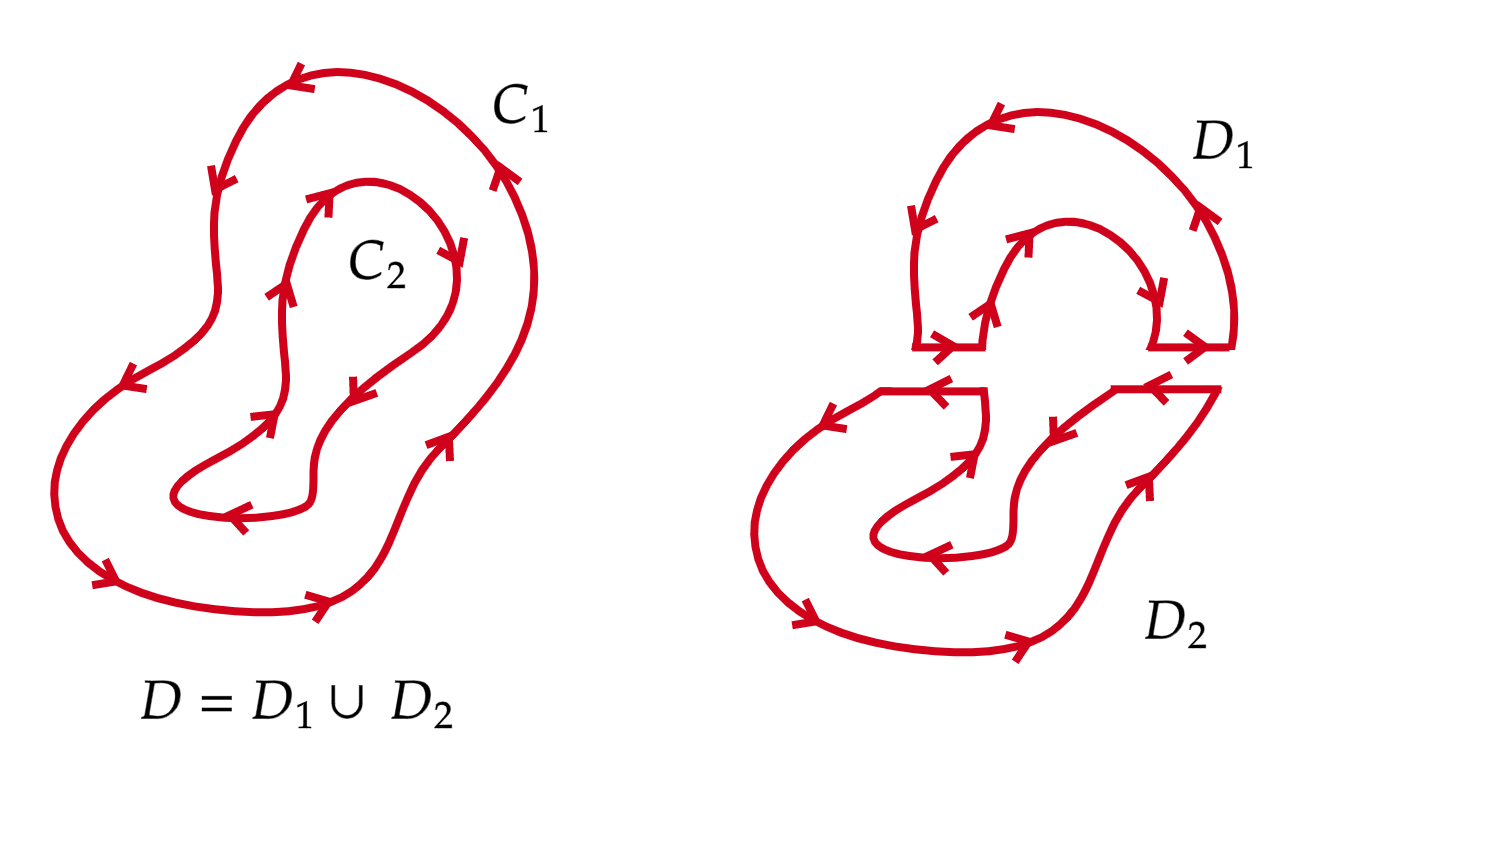
\includegraphics[width=\linewidth]{figures/wk-7/fig-2.png}
	\end{center}
\end{marginfigure}

\begin{ex}{Verifying Green's Formula by an Example}{label}
	We will verify Green's Formula for the vector field,
	\[\mathbf{F} = \frac{1}{2}(-y + x)\]
	where $D$  is taken to be the interior of the ellipse,
	\[\frac{x^2}{a^2}+\frac{y^2}{b^2}=1\]
	Parameterizing the curve gives that,
	\[\mathbf{c}(t)=(a \cos t, b \sin t) \quad \text{ where } \quad 0 \leq t \leq 2\pi\]
	Taking the derivative of $\mathbf{c}(t)$,
	\[\mathbf{c}^{\prime}(t) = (-a \sin \theta, b \cos \theta)\]
	Hence, $\mathbf{F}(\mathbf{c}(t)) \cdot \mathbf{c}^{\prime}(t) = \frac{1}{2} \cdot ab$ because,
	\[\mathbf{F}(\mathbf{c}(t)) = \left(\frac{1}{2} -b \sin \theta, \frac{1}{2} a \cos \theta\right)\]
	Integrating from $t = 0$ to $t = 2 \pi$ gives $ab \cdot \pi$. Thus,
	\[\oint_{\partial D^{+}} \mathbf{F} \cdot ds = \int_{0}^{2 \pi} \mathbf{F}(\mathbf{c}(t)) \cdot \mathbf{c}^{\prime}(t) dt = ab \cdot \pi\]
	On the other hand, 
	\[P(x,y) = -\frac{1}{2} \cdot y \quad \quad Q(x,y) = \frac{1}{2} \cdot x\]
	Computing the partial derivatives of $P$ and $Q$,
	\[P_y = -\frac{1}{2} \quad \quad Q_x = \frac{1}{2}\]
	It follows that,
	\[\iint_D (Q_x-P_y) d x d y = \iint_D \frac{1}{2} - \left(-\frac{1}{2}\right) d x d y = ab \cdot \pi\]
	since this integral is simply the area of an ellipse.
\end{ex}

\begin{ex}{Verifying Green's Formula by an Example}{label}
	We will verify Green's Formula on the line integral,
	\[\oint_{\mathbf{c}}\left(2 x^3-y^3\right) d x+\left(x^3+y^3\right) d y\]
	where $\mathbf{c}$ is the unit circle in the x-y plane oriented counter-clockwise. Taking $\mathbf{c}(t) = (\cos(t), \sin(t))$ for $0 \leq t \leq 2 \pi$,
	\[\oint_{\mathbf{c}} = \int_{0}^{2\pi} -2\cos^3t \cdot \sin t+\sin^4 t +\cos^4 t + \sin^3 t \cdot \cos t dt\]
	Applying the double angle formula, this evaluates to $\frac{3 \pi}{2}$. Now,
	\[Q_x = 3x^2 \quad \text{ and } P_y = -3y^2\]
	so $Q_x - P_y = 3(x^2 + y^2)$. In polar coordinates,
	\[\begin{aligned}
		\iint_D\left(Q_x-P_y\right) d x d y & =\int_0^{2 \pi} \int_0^1 3 r^2 \cdot r d r d \theta \\
		& = 2 \pi \int_0^1 3 r^2 d r \\
		& = \frac{3 \pi}{2}
		\end{aligned}\]
	where $r$ is the Jacobian.
\end{ex}

\hfill

\noindent A generalized formulation of Green's Theorem is that,

\hfill

\begin{thm}[Stokes' Theorem]
	Define the vector field,
	\[\mathbf{F}(x,y) = P(x,y) \cdot \mathbf{i} + Q(x,y) \cdot \mathbf{j}\]
	If $\mathbf{F}$ is continuously differentiable and defined on $D$, then,
	\[\oint_{{(\partial D)}^+} \mathbf{F} \cdot d \mathbf{s}=\iint_D(\nabla \times \mathbf{F}) \cdot \mathbf{k} d A\]
	where the \textbf{curl} of the vector field $\nabla \times \mathbf{F}$ represents its circulation.
\end{thm}

\begin{rmk}
	Fix a vector field $\mathbf{F}$ as,
	\[\mathbf{F}=P(x, y)\cdot\mathbf{i}+Q(x, y)\cdot\mathbf{j}\]
	Stokes' Theorem can be seen as generalizing Green's Theorem:
	\[\iint_S(\mathbf{\nabla} \times \mathbf{F}) \cdot d \mathbf{S}=\iint_S\left(Q_x-P_y\right) d x d y\]
\end{rmk}

\begin{rmk}
	For any two surfaces $S_1$ and $S_2$,
	\[\iint_{S_1}(\mathbf{\nabla} \times \mathbf{F}) \cdot d \mathbf{S}_1=\iint_{S_2}(\mathbf{\nabla} \times \mathbf{F}) \cdot d \mathbf{S}_2\]
	because Stokes' Theorem tells us that both integrals are equal to,
	\[\oint_{\mathbf{c}} \mathbf{F} d \mathbf{s}\]
	where $\left(\partial S_1\right)^{+}=\mathbf{c}=\left(\partial S_2\right)^{+}$
\end{rmk}

\begin{prop}
	If $S$ is a closed surface, then,
	\[\oiint(\underbrace{\mathbf{\nabla} \times \mathbf{F}}_{\mathbf{G}}) \cdot d \mathbf{S}=\mathbf{0}\]
	where $\mathbf{G}$ is called a \textbf{solenoidal vector field}.
\end{prop}

\begin{proof}
	Write $S = S_1 \cup S_2$ and split the integral:
	\[\oiint(\underbrace{\mathbf{\nabla} \times \mathbf{F}}_{\mathbf{G}}) \cdot d \mathbf{S}= \iint_{S_1} + \iint_{S_2} = \oint \mathbf{F} \cdot d \mathbf{S}_1+\oint \mathbf{F} \cdot d \mathbf{S}_2\]
	Exploiting the orientations of each component,
	\[\oint_{(\delta \mathbf{S}_1)^+} \mathbf{F} \cdot d \mathbf{S}_1+\oint_{(\delta \mathbf{S}_2)^+} \mathbf{F} \cdot d \mathbf{S}_2 = \oint_{(\delta \mathbf{S}_1)^+} \mathbf{F} \cdot d \mathbf{S}_1+ \oint_{(\delta \mathbf{S}_1)^-} \mathbf{F} \cdot d \mathbf{S}_2\]
	so we can cancel terms and obtain the desired integral.
\end{proof}

\begin{marginfigure}
	\begin{center}
	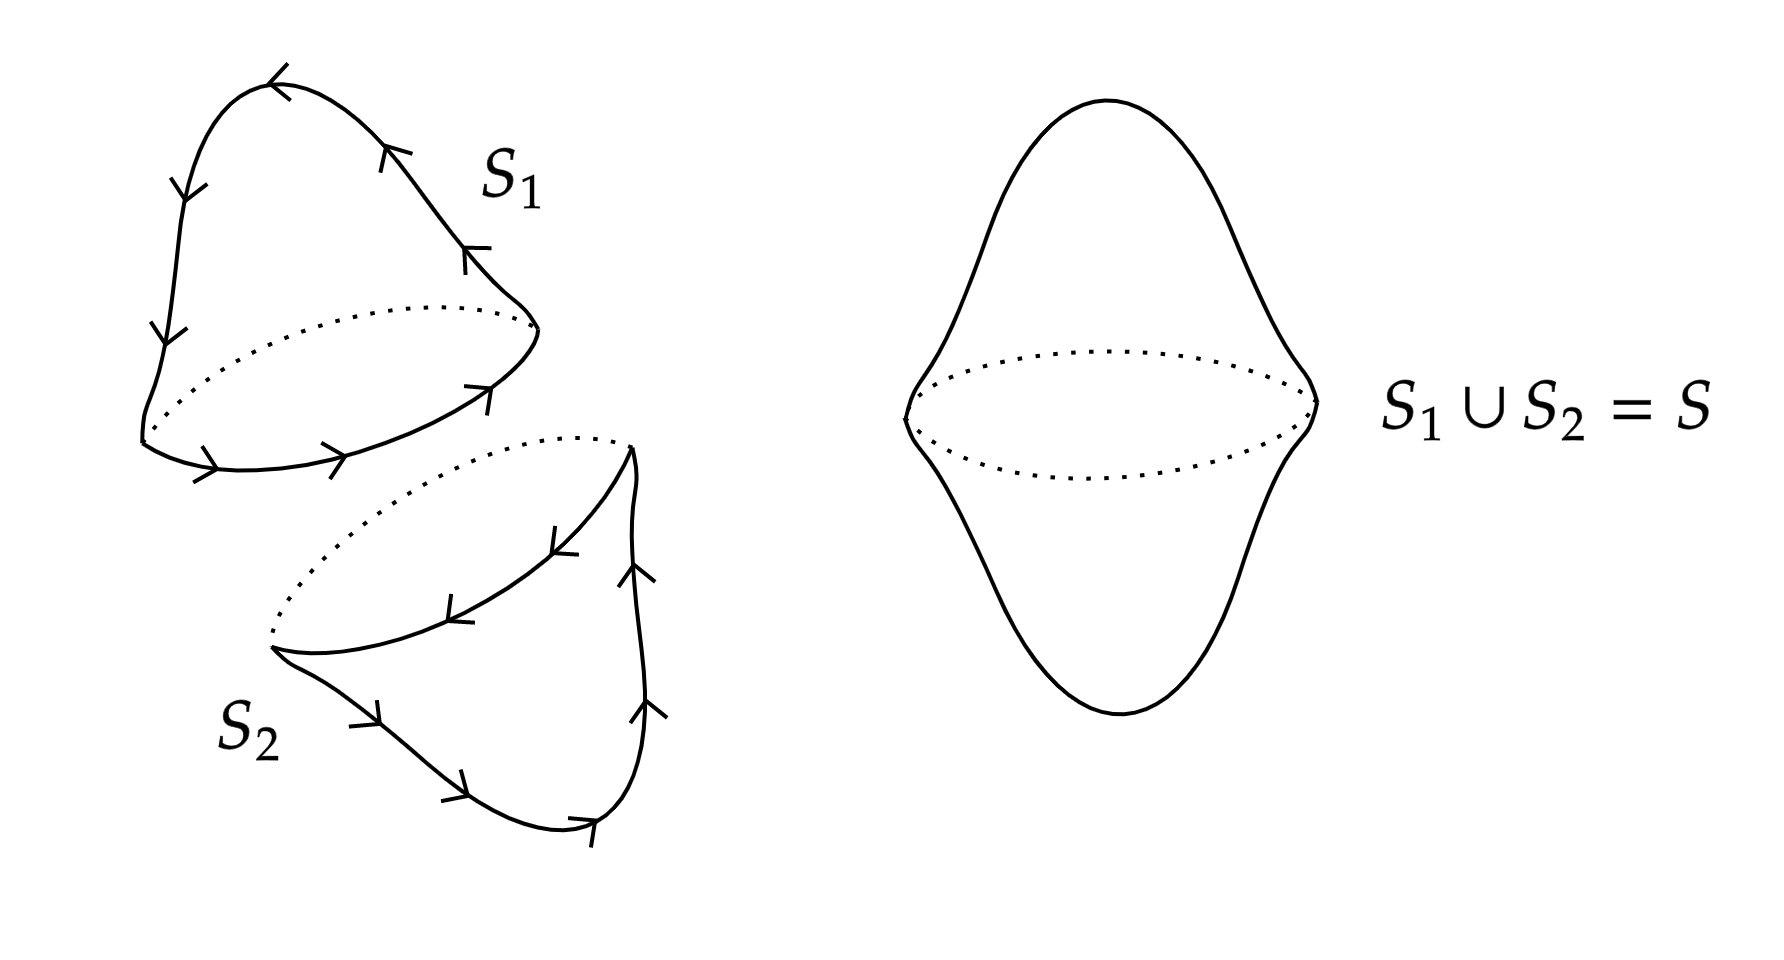
\includegraphics[width=\linewidth]{figures/wk-7/fig-4.png}
	\end{center}
\end{marginfigure}

\begin{cor}
	The net flux of a solenoidal vector field is always $0$.
\end{cor}

\subsection{Gauss' Divergence Theorem}
In this section, we will quantify the extent to which a vector field $\mathbf{F}$ fails to be solenoidal. Recall that a solenoidal vector field,
\[\mathbf{F} = \mathbf{\nabla} \cdot \mathbf{F} \neq 0\]
satisfies that $\mathbf{\nabla} \cdot \mathbf{F} = 0$.

\begin{thm}[Gauss' Divergence Theorem]
	Let $\mathbf{F}$ be a $C^1$ vector field in \text{$U \subseteq \R^3$}. Given a bounded open subset $V$ of $U$ where $\partial V$ is regular or piece-wise regular, 
	\[\oiint_{(\partial V)^+}\mathbf{F} \cdot d \mathbf{S}=\iiint_V(\mathbf{\nabla} \cdot \mathbf{F}) d x d y d z\]
	where the left-hand side is the flux of $\mathbf{F}$ across $(\partial V)^+$ and the right-hand side is the integral divergence of $\mathbf{F}$.
\end{thm}

\begin{marginfigure}
	Recall that the sign of $\mathbf{\nabla} \times \mathbf{F}$ is a measure of the contraction or expansion of the flow lines of $\mathbf{F}$. Specifically,
	\begin{align*}
		&\mathbf{F} < 0 \implies \text{Contraction} \\
		&\mathbf{F} > 0 \implies \text{Expansion} \\
	\end{align*}
\end{marginfigure}

\begin{thm}[Gauss' Law]
	Consider the vector field
	\[\mathbf{F}=\frac{\mathbf{r}}{\|\mathbf{r}\|^3} \quad \text{ where }\quad \mathbf{r}=x \cdot \mathbf{i}+y \cdot \mathbf{j}+z \cdot \mathbf{k}\]
	Observe that the norm of $\mathbf{F}$ is,
	\[\|\mathbf{F}\|=\left\|\frac{\mathbf{r}}{\|\mathbf{r}\|^3}\right\|=\left\|\frac{1}{\|\mathbf{r}\|^3}\right\| \cdot\|\mathbf{r}\|=\frac{1}{\|\mathbf{r}\|^2}=\frac{1}{x^2+y^2+z^2}\]
	defined on $U = \R^3 - \{\mathbf{0}\}$. 
	\[
	\oiint_{S_1} \mathbf{F} \cdot d \mathbf{s} =
	\begin{cases}
		4 \pi & \text{ if } \mathbf{0} \not\in S_2 \\
		0 & \text{ if } \mathbf{0} \in S_2
	\end{cases}
	\]
\end{thm}

\begin{marginfigure}
	To prove Gauss' Law, fix a sphere at the origin and apply the Divergence Theorem to the region between the sphere and the surface.
\end{marginfigure}

\begin{defn}[Outgoing Flux]
	The \textbf{outgoing flux} of a vector field $\mathbf{F}$ is,
	\[\int_{(\partial D)^{+}} \mathbf{F} ds = \int_{a}^{b} \mathbf{F}(\mathbf{c}(t)) \cdot \mathbf{n}(t) dt\]
	where $\mathbf{n}(t) = (y^{\prime}(t), -x^{\prime}(t))$.
\end{defn}

\begin{rmk}
	The outgoing flux of $\mathbf{F}$ across $(\partial D)^+$ satisfies,
	\[\int_{(\partial D)^{+}} \mathbf{F} ds = \iint_D(\mathbf{\nabla} \cdot \mathbf{F}) d x d y\]
\end{rmk}

\begin{proof}
	Since $\mathbf{F} = P(x,y) \cdot \mathbf{i} + Q(x,y) \cdot j$,
	\begin{align*}
		\int_a^b \mathbf{F}(\mathbf{c}(t)) \cdot \mathbf{n}(t) d t&=\int_a^b(P \mathbf{i}+Q \mathbf{i}) \cdot\left(y^{\prime}(t), x^{\prime}(t)\right) d t \\
		&= \int_{(\partial D)^{+}}-\underbrace{P}_{\tilde{P}} d x+ \underbrace{Q}_{\tilde{Q}} d y \\
		&=\iint_D(P_x+Q_y) d x d y \\
		&= \iint_D(\mathbf{\nabla} \cdot \mathbf{F}) d x d y
	\end{align*}
\end{proof}